\subsection{Stability and Time-Step Efficiency}
\label{subsec:stability_time_step}

\subsubsection{Stability Analysis}

To assess the stability of the time-integration methods, the
semi-discrete system was expressed in matrix form as
\begin{equation}
    \frac{d\mathbf{T}}{dt}
    =
    \mathbf{A}\mathbf{T}+\mathbf{b},
    \label{eq:semi_discrete_matrix}
\end{equation}
where $\mathbf{A}$ represents the linear spatial discretization,
including the contributions of the boundary conditions, and
$\mathbf{b}$ contains the temperature-independent source terms.
Since the prescribed velocity field makes the viscous-dissipation
source independent of temperature, it does not affect the
eigenvalue-based stability analysis.

The eigenvalues of $\mathbf{A}$ were computed numerically for
the $50\times20$ grid. The maximum real part and maximum
eigenvalue magnitude were found to be
\begin{equation}
    \max_k \Re(\lambda_k)
    =
    -1.216672\times10^{1},
    \qquad
    \max_k |\lambda_k|
    =
    1.142857\times10^{2}.
\end{equation}
The negative real parts indicate that the semi-discrete system
is asymptotically stable.

The absolute stability of a time-integration method can be
examined by applying it to the scalar test equation
$\dot{w}=\lambda w$. Defining $z=\lambda\Delta t$, the
numerical solution takes the form
$w^{n+1}=G(z)w^n$, where stability requires
$|G(z)|\leq1$. The amplification factors for the methods
considered here are
\begin{align}
    G_{\mathrm{IE}}(z)
    &=\frac{1}{1-z},
    \\
    G_{\mathrm{RK2}}(z)
    &=1+z+\frac{z^2}{2},
    \\
    G_{\mathrm{RK4}}(z)
    &=1+z+\frac{z^2}{2}
      +\frac{z^3}{6}+\frac{z^4}{24},
\end{align}
for implicit Euler, explicit midpoint RK2, and classical
explicit RK4, respectively. For a given time step, the
stability condition is evaluated over the computed spectrum:
\begin{equation}
    \max_k \left|G(\lambda_k\Delta t)\right|
    \leq 1.
    \label{eq:modal_stability_condition}
\end{equation}

Implicit Euler is A-stable and therefore stable for the
computed spectrum, since all eigenvalues have negative
real parts. In contrast, the explicit methods have
conditional stability, and their allowable time steps
depend on the eigenvalue distribution. The maximum stable
time step for each method was estimated numerically using
the search procedure presented in
Algorithm~\ref{alg:maximum_stable_timestep}.

\begin{algorithm}[htbp]
    \caption{Numerical estimation of the maximum stable time step}
    \label{alg:maximum_stable_timestep}
    \small
    \begin{algorithmic}[1]
        \Require Eigenvalues $\{\lambda_k\}$, integration scheme,
                 initial time step $\Delta t_0$
        \Ensure Estimated maximum stable time step

        \State $\alpha \gets \max_k \Re(\lambda_k)$

        \If{$\alpha > \text{stability tolerance}$}
            \State \Return NaN
            \Comment{The semi-discrete system is unstable}
        \EndIf

        \If{scheme is implicit Euler}
            \State \Return $\infty$
            \Comment{Implicit Euler is A-stable}
        \EndIf

        \State $\Delta t_{\mathrm{low}} \gets 0$
        \State $\Delta t_{\mathrm{high}} \gets
               \max(\Delta t_0,10^{-12})$
        \State bracketed $\gets$ False

        \Comment{Bracket the stability boundary}
        \For{$m=1,\ldots,N_{\mathrm{double}}$}
            \If{$\max_k |G(\lambda_k\Delta t_{\mathrm{high}})|>1$}
                \State bracketed $\gets$ True
                \State \textbf{break}
            \EndIf
            \State $\Delta t_{\mathrm{low}}
                   \gets \Delta t_{\mathrm{high}}$
            \State $\Delta t_{\mathrm{high}}
                   \gets 2\Delta t_{\mathrm{high}}$
        \EndFor

        \If{not bracketed}
            \State \Return $\infty$
            \Comment{No instability found within the search range}
        \EndIf

        \Comment{Refine the boundary by bisection}
        \For{$m=1,\ldots,N_{\mathrm{bisect}}$}
            \State $\Delta t_{\mathrm{mid}}
                   \gets \frac{1}{2}
                   (\Delta t_{\mathrm{low}}+
                   \Delta t_{\mathrm{high}})$
            \If{$\max_k |G(\lambda_k\Delta t_{\mathrm{mid}})|
                  \leq 1$}
                \State $\Delta t_{\mathrm{low}}
                       \gets \Delta t_{\mathrm{mid}}$
            \Else
                \State $\Delta t_{\mathrm{high}}
                       \gets \Delta t_{\mathrm{mid}}$
            \EndIf
        \EndFor

        \State \Return $\Delta t_{\mathrm{low}}$
        \Comment{Return the stable side of the estimated limit}
    \end{algorithmic}
\end{algorithm}

At the configured time step $\Delta t=0.1$, the maximum
amplification factors were $0.45113$, $54.87755$, and
$516.90726$ for implicit Euler, RK2, and RK4, respectively.
Thus, implicit Euler was stable at this time step, whereas
both explicit methods were unstable. The numerical search
estimated maximum stable time steps of $0.01750$ for RK2
and $0.0243713$ for RK4. The estimated stability limit of
RK4 is therefore greater than that of RK2 for the present
spatial discretization.

The results are summarized in
Table~\ref{tab:maximum_timestep}. The implicit Euler method
has no finite absolute-stability limit for the computed
spectrum. The AFI value represents the largest tested
convergent time step, rather than a theoretically established
stability bound. The eigenvalue-based stability analysis
for implicit Euler should also not be interpreted as a
formal stability result for AFI, which uses approximate
factorization and was assessed separately through numerical
convergence tests.

\begin{table}[htbp]
    \centering
    \small
    \caption{Stability limits and selected pseudo-time steps
    for the numerical methods.}
    \label{tab:maximum_timestep}
    \begin{tabular}{@{}l c p{3.0cm} p{5.0cm}@{}}
        \hline
        Method
        & $\max_k |G|$ at $\Delta t=0.1$
        & Maximum stable or selected $\Delta t$
        & Assessment
        \\
        \hline
        AFI
        & --
        & $0.271$ (largest tested)
        & Largest tested value for which convergence was obtained.
        \\[0.1cm]
        Direct implicit Euler
        & $0.45113$
        & No finite stability limit; $1.0$ selected
        & A-stable for the computed eigenvalue spectrum.
        \\[0.1cm]
        Explicit RK2
        & $54.87755$
        & $0.01750$ (estimated)
        & Conditionally stable; unstable at $\Delta t=0.1$.
        \\[0.1cm]
        Explicit RK4
        & $516.90726$
        & $0.0243713$ (estimated)
        & Conditionally stable; unstable at $\Delta t=0.1$.
        \\
        \hline
    \end{tabular}
\end{table}

For the direct implicit solver, a representative time step
of $\Delta t=1$ was selected for the efficiency comparison.
This choice is substantially more moderate than the very
large values identified in the preliminary time-step sweep.
It is nevertheless expected to provide strong modal damping.
In particular, for backward Euler and the computed spectrum,
\begin{equation}
    \max_k |G_{\mathrm{IE}}(\lambda_k\Delta t)|
    \leq
    \frac{1}{1-\Delta t\max_k\Re(\lambda_k)}.
\end{equation}
At $\Delta t=1$, this gives
\begin{equation}
    \max_k |G_{\mathrm{IE}}(\lambda_k)|
    \leq 0.07595.
\end{equation}
The selected time step must still be checked through the
steady-state residual to verify convergence.

These stability limits concern pseudo-time integration
toward the steady solution and do not establish the accuracy
of a physical transient simulation.

\subsubsection{Time-Step Efficiency}

A time-step efficiency study was performed for AFI and the
direct implicit solver on the $50\times20$ grid. Several
candidate time steps were tested for each method, with
three independent runs per candidate. Each run started
from the initial temperature field and was considered
converged when the steady-state residual satisfied the
prescribed tolerance of $10^{-12}$. All tested cases in
the preliminary study converged in all three runs.

For AFI, the fastest tested case used
$\Delta t=0.266$, with a median computation time of
$5.6624~\mathrm{s}$, 296 iterations, and a final residual
of $9.51\times10^{-13}$. Its runtime was only marginally
lower than that obtained with $\Delta t=0.265$, indicating
a relatively shallow minimum in the tested range rather
than a precisely established optimal time step.
Figure~\ref{fig:afi_timestep_efficiency} shows the
computation time across the tested AFI time steps.

\begin{figure}[htbp]
    \centering
    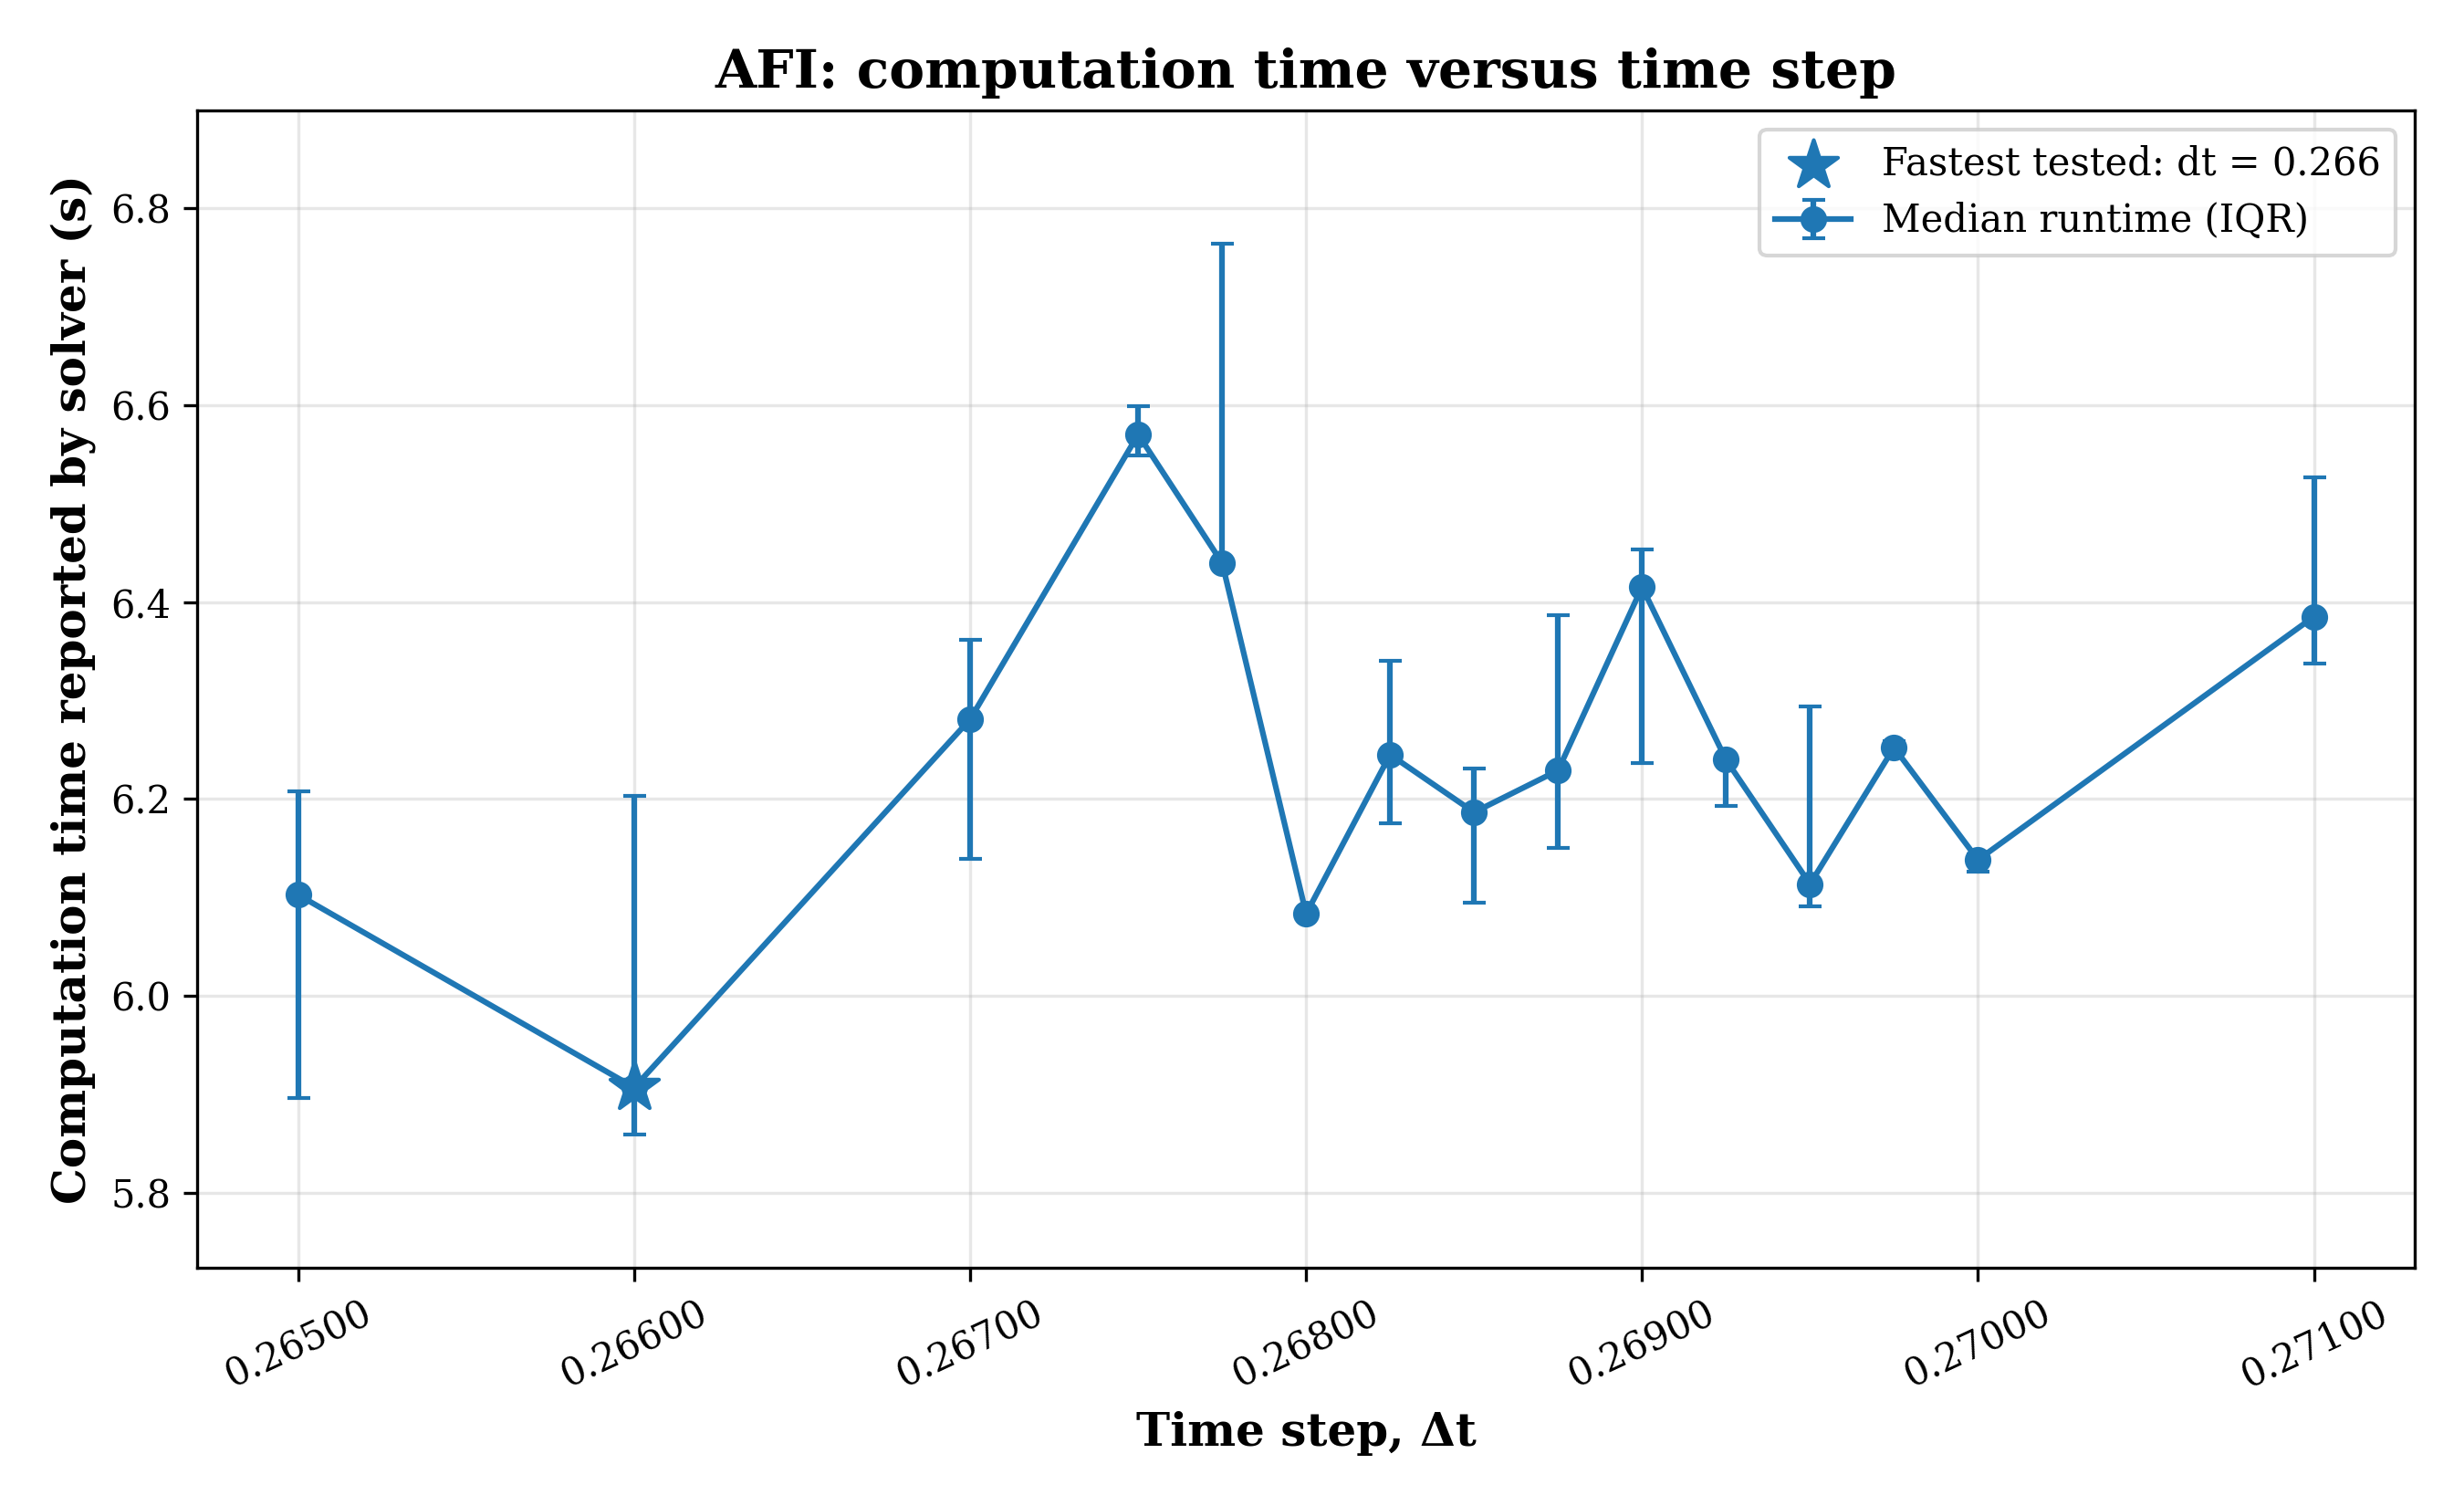
\includegraphics[width=0.85\textwidth]
    {figures/runtime_vs_dt_AFI.png}
    \caption{Median computation time of AFI as a function
    of the pseudo-time step. The minimum among the tested
    values occurs at $\Delta t=0.266$.}
    \label{fig:afi_timestep_efficiency}
\end{figure}

For the direct implicit solver, the representative value
$\Delta t=1$ was selected instead of the very large
time step that produced the minimum runtime in the
preliminary sweep. The preliminary sweep identified
$\Delta t=20000$ as its fastest tested case, but this
extremely aggressive pseudo-time step was not retained
for the comparison. The direct solver must therefore be
rerun at $\Delta t=1$ to determine its median computation
time, iteration count, and final residual. These results
will be used to assess its practical efficiency alongside
AFI under the selected settings.

\subsubsection{Comparison of the Converged Solutions}

To verify that the two solvers produce the same
steady-state solution, their temperature fields at the
selected time steps should be compared over the physical
cells, excluding ghost cells. The relative $L_2$ difference
is defined as
\begin{equation}
    \varepsilon_{\mathrm{AFI,Direct}}
    =
    \frac{
    \left\|
    \mathbf{T}_{\mathrm{AFI}}
    -
    \mathbf{T}_{\mathrm{Direct}}
    \right\|_2
    }{
    \left\|
    \mathbf{T}_{\mathrm{Direct}}
    \right\|_2
    }.
    \label{eq:afi_direct_relative_difference}
\end{equation}
This quantity should be recalculated using the direct
solution obtained with $\Delta t=1$. The previously
obtained value of $1.15\times10^{-14}$ corresponds to
the direct-solver run at $\Delta t=20000$ and is therefore
not reported as the result of the revised comparison.

The computation-time comparison should likewise use the
new direct-solver measurement at $\Delta t=1$. Since the
direct solver's runtime and iteration count can change
with the selected time step, no speedup ratio is reported
until the revised run has been completed. Any resulting
performance comparison remains specific to the present
grid, problem configuration, and implementation.